\section{Problem Definition}
\label{sec:problem}

\begin{figure}[t]
\centering
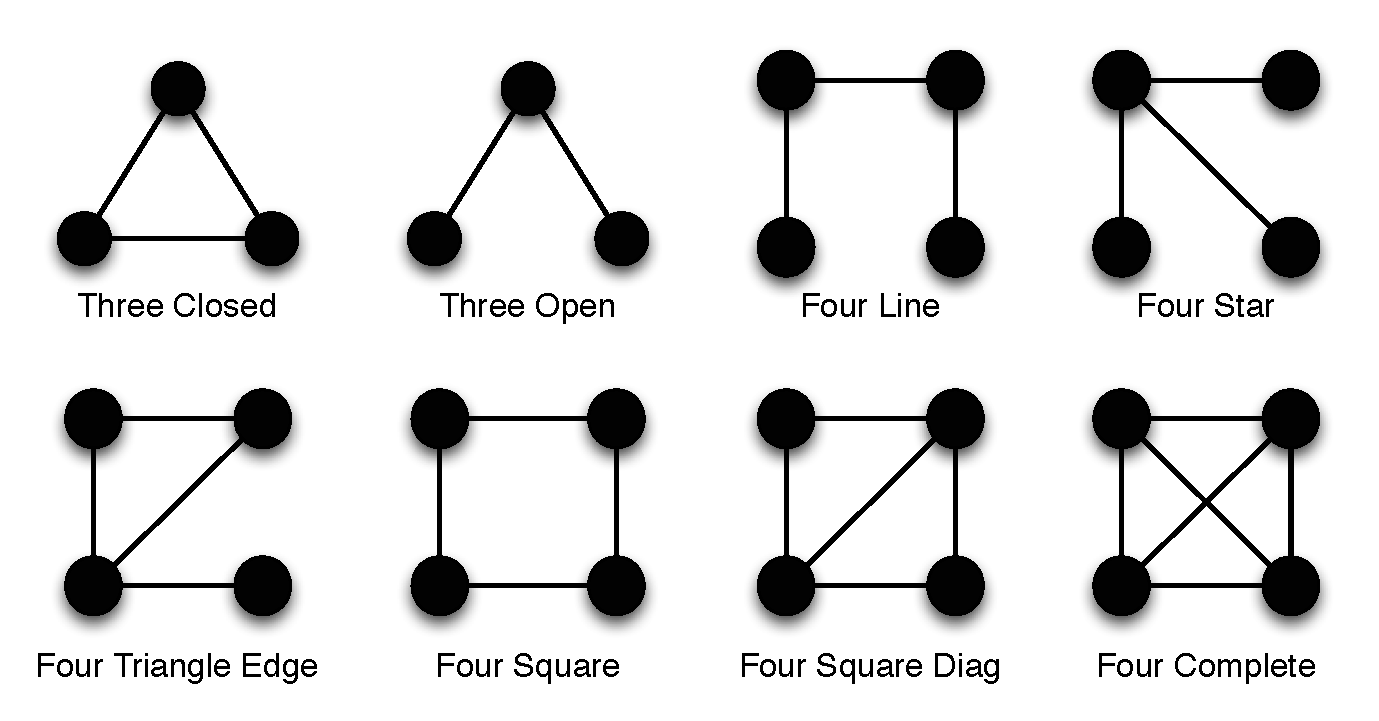
\includegraphics[width=3in]{Figures/motifs.eps}
\caption{Graphical representation of the 3-motif and 4-motif.}
\label{fig:motif}
\end{figure}

In this section, we first give some basic concepts that we use throughout in the paper. Then, we present formulate the problem of motif-driven graph generation problem. 

\textbf{Graph} is a representation of a set of objects and correlations or connections between them. The objects in graph called nodes and the relations called edges. Let $G = (V, E)$ be a graph, where $V$ is a set of $|V| = N$ nodes and $E \subseteq V \times V$ is a set of correlations or connections between nodes. A graph without a self-loop or multi-edge is called simple graph. Without loss of generality, we assume the graph is simple, connected and undirected.

\textbf{Subgraph} is a graph $G' = (V', E')$ whose nodes $V'$ and edges $E'$ form subsets of the graph nodes $V(V' \in V)$ and edges $E(E' \in E)$of a given graph $G = (V, E)$. In graph $G'$, if $V' \in V, E' \in E$ and $\{e = (v_a, v_b) : v_a, v_b \in V, e \in E, e \not\in E'\}$ then $G'$ is a \textbf{vertex-induced subgraph(induced subgraph)}.

\textbf{Motif} is defined as a small, connected, non-isomorphic, induced subgraph of graph. In this paper, we only use 8 motifs within k nodes, where $k \in \{3, 4\}$. We use \textit{k}-motif as a motif with $k$ nodes. Here, we have ThreeClosed, ThreeOpen of \textit{3}-motif, and FourLine, FourSquare, FourStar, FourTriangleEdge, FourSquareDiag and FourComplete of \textit{4}-motif which show in Figure~\ref{fig:motif}

\emph{Problem } \textbf{Motif-driven graph generation.} 
\vpara{Input: } The input of our problem consists of two components, i.e., the basic attributes $|V|$ and $|E|$ of the network $G$ and the motif distribution $D$ of graph $G$, where $D$ only contains the motifs we mentioned in Figure~\ref{fig:motif}. 

\vpara{Output: } Our goal is to generate a graph $G'$ which has the same basic attributes as $G$ and approximate motif distribution as $D$.

The problem formulation is different from the traditional graph generation problem \cite{erdds1959random, watts1998collective, albert2002statistical, newman2009random, molloy1995critical}, as in this paper we focus on generating graph based on the motif distribution. Since in social science domain, the distribution of motif is highly used for analyzing large graphs and it's a like basic property.



